%HEVEA \begin{bgcolor}{cyan}
%HEVEA \color{Red}
\chapter{Detailed Help on usage}
%HEVEA \end{bgcolor}
%HEVEA \begin{bgcolor}{SpringGreen}
%HEVEA \color{black}
\section{Starting RLTOOL}
%HEVEA \end{bgcolor} 
Load the rltool library as per instructions in the README file. If the
library loads properly the following message is displayed on Scilab prompt: 

%HEVEA \begin{bgcolor}{Gray}
%HEVEA \color{black}
\begin{center}
{\tt
mode(-1); \\
rltool is loaded. Type "rlt()" to start rltool-1.6\\              
}
\end{center}
%HEVEA \end{bgcolor} 
Type ``rlt()'' to start this programme. 
%HEVEA \begin{bgcolor}{SpringGreen}
%HEVEA \color{black}
\section{Rootlocus}
%HEVEA \end{bgcolor} 
\label{rootlocus}
On typing ``rlt()'', the you will be  prompted to either select a new
rltool session or load a previous saved file. If a new session is
selected, the you will be  prompted to enter the transfer
function as numerator / denominator in the variable '$s$'. Rltool will
automatically load the plant you were working with in the previous
session of rltool. Click ``Ok'' to confirm this plant. You may wish to
edit the plant, in that case type in the new plant and click ``Ok''. 

A Rootlocus plot of the transfer function is displayed. Open loop
poles are shown by crosses and zeros by circles. 
%BEGIN IMAGE
\begin{figure}
\centerline{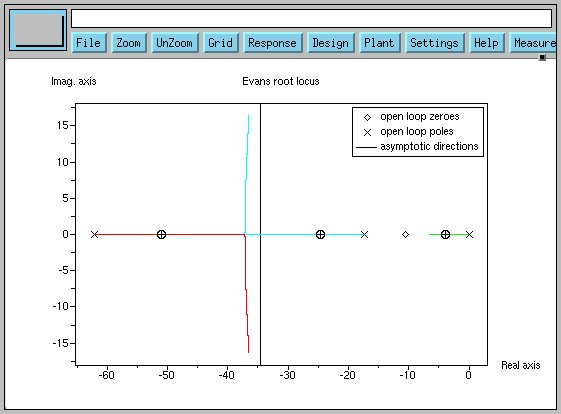
\includegraphics[width=3 in]{Rlt_main}}
\caption{Rltool main window}
\label{Rlt_main}
\end{figure}
%END IMAGE
%HEVEA\imageflush
This window is shown in Figure (\ref{Rlt_main}). The various menus in
the window are:
%HEVEA \begin{bgcolor}{Gray}
%HEVEA \color{black}
\begin{enumerate}
\item ``File'': Load, save or print the rootlocus.
\item ``Zoom'': Select a part of the rootlocus using the mouse and
  zoom onto it.
\item ``UnZoom'': See the entire rootlocus (remove Zoom, if any).
\item ``Grid'' : Menus under this head control the apperance of grids
  on all plots. These are:
%HEVEA \begin{bgcolor}{SpringGreen}
  \begin{enumerate}
    \item ``On'': Put a cartesian grid on all plots in the current
    session.
    \item ``Off'': Remove (if already present) a cartesian grid from
    all plots in the  current session.
    \item ``Zeta/Wn'': Plot a constant $\zeta$ and $\omega_n$ curve on
    the rootlocus for a given value of $\zeta$ and $\omega_n$.
    \item ``sgrid'': Plot a constant $\zeta$ and $\omega_n$ grid on
    the rootlocus.
  \end{enumerate} 
%HEVEA \end{bgcolor}
\item ``Response'': Various plots and responses can be viewed. 
 
%HEVEA \begin{bgcolor}{SpringGreen}
 \begin{enumerate}
\item ``Closed loop'': Closed loop responses for a given gain. More
  details are given in Section \ref{closedloop}.
\item ``Nyquist'': Nyquist plot.
\item ``Nichols'': Nichols chart.
\item ``Details'': Numerical values of poles and zeros, gain etc.
\item ``Popov'': The Popov-plot of the system.
\end{enumerate}
%HEVEA \end{bgcolor}
\item ``Design'': There are two modes available in Rltool, namely
  Rootlocus and Frequency.
 %HEVEA \begin{bgcolor}{SpringGreen}
 \begin{enumerate}
    \item ``Root Locus'': This is the default mode. Most options here
    are with a view towards time-domain design.
    \item ``Frequency'': This mode is still under
    development. Currently very limited options are available, like
    bode plots, sensitivity plots etc. 
  \end{enumerate}
%HEVEA \end{bgcolor}
\item ``Plant'': This menu provides utilities for editing the
  system. More details are given in Section \ref{plant}.
\item ``Save'': Save the current session and/or load previous
  sessions.
\item ``Settings'': This menu provides all settings available to the
  user. More details are given in Section \ref{settings}.
\item ``Help'': A short online help is included on most topics. Click
  the sub-menu under this head to see the help. For example, help on
  rootlocus is included in ``Help\rar Root Locus''. 
\item ``Measure'': This feature allows a user to ``measure'' the gain
  at a point on the rootlocus. The user is first prompted to select a
  point. If this point is on the rootlocus, relevant information is
  displayed/updated. 
\end{enumerate}
%HEVEA \end{bgcolor}
%HEVEA \begin{bgcolor}{SpringGreen}
\section{The control center}
%HEVEA \end{bgcolor}
Immediately after starting rltool, a user will see the control center
GUI.
%BEGIN IMAGE
\begin{figure}
\centerline{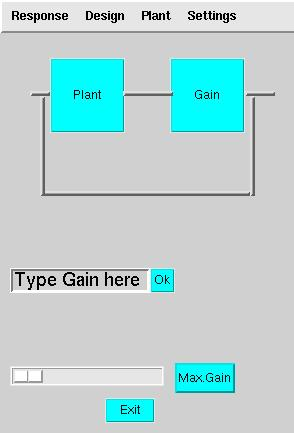
\includegraphics[width=2 in]{Rlt_GUI}}
\caption{The control center}
\label{Rlt_GUI}
\end{figure}
%END IMAGE
%HEVEA\imageflush
A user can use and configure most features using this simple
GUI. Following is a brief description of features:
%HEVEA \begin{bgcolor}{Gray}
\begin{enumerate}
\item Menus: Menus are mostly similar to the ones described in Section
  \ref{rootlocus}.
\item ``Plant'' button: Click on this button to edit the current
  transfer function.
\item ``Gain'' button: This displays the current gain selected by the
  user.
\item Gain set (text mode): This field displays a message ``Type Gain
  Here'' by default. A user can type in a positive real valued gain in
  this field. Click on ``Ok'' to load this gain into Rltool. 
\item Slider: A user can select gain with a slider. The value of the
  gain selected is shown immediately above the slider.
\item Max. Gain: This popup menu lets a user select the maximum
  allowed gain for the rootlocus. Options are 10, 50, 100,
  500,...100,000. A user may also set the maximum allowed gain to a
  different value using the Settings menu. 
\item Exit button: Click on this button to quit rltool. 
\end{enumerate} 
%HEVEA \end{bgcolor}
The most convenient way to use Rltool is to set a gain using the
slider. The current gain is displayed above the slider bar and also in
the ``gain'' button on the control center. Also, a window containing
the following closed loop plots is continuously updated:
%HEVEA \begin{bgcolor}{Gray}
\begin{enumerate}
   \item Closed loop pole(s) and zero(s)
   \item Closed loop unit step response.
   \item Closed loop bode plot.
   \item Sensitivity plot
\end{enumerate}
%HEVEA \end{bgcolor}
Note that ``closed loop plant'' may include either ``gain in feedback'' or
``gain in forward path''. Please see the ``Settings'' section for how to
do this. A user can also set the units (hz or rad/sec) for  bode and
sensitivity plots. Please see the section on "Settings". 

%A user can view the exact (numerical value) of closed loop poles, zeros
%and gain by clicking on ``Response \rar Details''. A popup window displays
%this data. Click on "step response" button of the popup window to view
%data like damping factor, overshoot, rise time etc. The damping
%factor is computed for a dominant pole   approximation. 

%If you want a grid on the rootlocus, select ``Grid \rar  On''. Likewise,
%to turn it off, select ``Grid \rar  Off''. If you want to draw constant
%damping ratio $\zeta$ and natural frequency $\omega_n$ lines,
%click on ``Grid \rar Zeta/Wn''. You will be prompted to enter one
%$\zeta$ and one $\omega_n$ of your choice. If you want to do this for
%various values of $\zeta$ and $\omega_n$ try ``Grid \rar sgrid''.

%The rootlocus is plotted with a finite (maximum) gain. This is, by
%default set to 1000. You can change this by clicking on ``Settings
%\rar Rootlocus''. You might want to increase/decrease the maximum possible
%gain if your rootlocus shows hanging/incomplete lines or is too
%cluttered. Keeping this gain more than $1\times e^{10}$ may result in
%errors. 
%HEVEA \begin{bgcolor}{SpringGreen}
\section{Frequency design}
%HEVEA \end{bgcolor}
Rltool comes with two design modes... time domain (rootlocus) and
frequency domain. You can select the frequency domain mode by clicking
on ``Design \rar Frequency''. You will see the frequency magnitude plot
of the open loop transfer function. The magnitude is shown in decibel
and frequency in rad/sec. Click on the plot to determine the magnitude
and frequency. The frequency domain part is still under
development. It will be a great idea to take up this aspect and design
it further! You can ofcourse return to the rootlocus mode by clicking
on ``Design \rar  Root Locus''.
%HEVEA \begin{bgcolor}{SpringGreen}
\section{Editing of Plants}
%HEVEA \end{bgcolor}
\label{plant}
These utilities are provided under the ``Plant'' tab on the main window.
In the Root Locus mode, you can edit your plant at the click of a
mouse. The following options are provided. The function of most of
these should be obvious:
%HEVEA \begin{bgcolor}{Gray}
\begin{enumerate}
\item Undo: Undo one change in the (open loop) plant.
\item Add pole: Select the pole to be added by clicking on the
graphics window. If you select a point with nonzero real part, both
the point and its complex conjugate are added. That is, if $G(s)$ is
the current open loop transfer function and you select a complex point
$z$, the new open loop plant will be 
\[
G(s)\times \frac{1}{(s-z)(s-z^*)}
\]
where $z^*$ denotes the complex conjugate of $z$.
\item Remove pole: Click on the open loop pole that you want to
remove. If you click on a pole with nonzero real part, both the pole
and its complex conjugate are removed. 
\item Add zero: Similar to Add pole. Zero(s) are added to open loop
transfer function.
\item Remove zero: Similar to Remove pole. Zero(s) are removed from
the open loop transfer function.
\item Add cascade: You will be prompted to enter a transfer function 
$H(s)=a(s)/b(s)$. If $G(s)$ is the current transfer function, it is
modified to
\[G(s)\times H(s)\]
You will be prompted to ``accept'' this product. You can edit it if
you wish (to truncate some spurious decimal places etc). This command
is like a simultaneous addition of pole(s) and zero(s). However, in
this case you are required to enter these through the keyboard,
instead of using the mouse for the selection.
\item Remove cascade: is like dividing $G(s)$ by $H(s)$, i.e. the open
loop plant is modified to 
\[\frac{G(s)}{H(s)}\]
\item Edit plant: The current plant is displayed in a dialogue
box. You can modify it directly by typing in the appropriate value.
\end{enumerate}
%HEVEA \end{bgcolor}
%HEVEA \begin{bgcolor}{SpringGreen}
\section{Closed loop responses}
%HEVEA \end{bgcolor}
\label{closedloop}
There is a great deal of flexibility in rltool to see various closed
loop responses. First you will have to select one ``gain configuration'' out of
the possible two. Click on ``Settings \rar Gain Configuration''. You will
see a selection dialogue box with two choices:

You can choose the gain to be in the forward path as shown in the figure.
%BEGIN IMAGE
\begin{figure}
\centerline{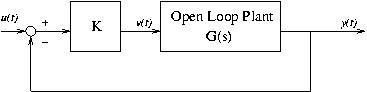
\includegraphics[width=3 in]{closedloop}}
\caption{K in forward path}
\end{figure}
%END IMAGE
%HEVEA\imageflush

This corresponds to the option ``K in forward path''. You can choose
to put ``K in the feedback path''. However, ``K in forward path'' is
the default. 

To see closed loop responses, click on ``Response \rar Closed Loop''. You
will be prompted to click on a point of the rootlocus to select the
``operating point'' at which you want to see the closed loop
response. Once you select the operating point, you are done! 

Rltool calculates the closed loop transfer function for the
configuration you have selected, i.e. the closed loop transfer
function for ``K in forward path'' is
\[ \frac{G K}{1+G K} \]
and the closed loop transfer function for ``K in feedback path'' is
\[ \frac{G}{1+GK}\]
You will see a selection menu that shows the following:
%HEVEA \begin{bgcolor}{Gray}
\begin{enumerate}
\item The gain corresponding to operating point you selected.
\item Whether the closed loop system is stable or unstable.
\item Impulse response: Click here to see the impulse response!
\item Step response selection: Unit step response is displayed. A
``details'' button in the step response also displays parameters such
as percent overshoot, rise time, settling time, $\zeta$ corresponding
to second order approximation etc.
\item Ramp response: Unit ramp response.
\item Arbitrary input: You can enter piece-wise linear, single valued
inputs through a graphics window. Use the mouse (press left button and
drag) to ``draw'' this input. There are a host of features like
``undo'', ``abort'' etc which can be used. You can also resize your
window to suit the range of your input. Click ``Edit \rar Ok'' when you are
done. If your input is single-valued, you will see the response of the
closed loop system to this input. 
\item Sinusoidal input: The input is of the form
\[A sin (\omega t)\]
Output is simulated, by default for one of the input and is
plotted. The default settings are $A=1$ and $\omega=1 \,
rad/sec$. These can be changed by clicking on ``Settings'' button in
the sinusoidal response window. You must close this window to return
to the response selection menu.
\item Frequency response (bode plot) of closed loop system. There is a
choice in the units (Rad/sec) or (Hz). These are available in
``Options'' menu in the frequency response window. 
\item Sensitivity plot: Sensitivity is defined as the transfer
  function between the input $u(t)$ and the {\it error} $e(t)$. For
  the system shown in the above figure, the sensitivity can be found
  to be 
\[\frac{1}{1+kG(s)} \]
This transfer function is evaluated on the imaginary axis (by
substituting $s=i\omega$) and the resulting (magnitude) plot is shown
for various values of $\omega$.  Options are similar to above. 
\end{enumerate}
Click on ``cancel'' to close the response selection menu and return to
the main window of rltool. 
%HEVEA \end{bgcolor}
%HEVEA \begin{bgcolor}{SpringGreen}
\section{Other responses}
%HEVEA \end{bgcolor}
\subsection{Nyquist plot} 
Nyquist plot of the open loop plant $G(s)$ can be seen by clicking on
``Response \rar Nyquist''. The gain and phase margin is displayed on the
plot. If you find that your plot is too coarse or cluttered, you can
change the minimum and maximum frequency in
``Settings \rar Nyquist-Nichols plot''. The frequency units can be
changed in ``Settings \rar Frequency units''. 

\subsection{Nichols plot}
Nichols plot for $G(s)$ is obtained by selecting
``Response \rar Nichols''. If the grid (in the main menu) is set to
``on'' you will see the logarithmic grid superimposed on the Nichols
plot. Here too, you can select the desired frequency units. 
\subsection{Popov plot}
The Popov plot can be used to predict the stability of the closed loop
system with a sector bound nonlinearity in loop. We plot real part of
$G(i\omega)$ on the real axis and $\omega {\rm Imaginary} \,
G(i\omega)$  on the imaginary axis. A simple construction then gives
the range of the ``Popov sector'' and the ``multiplier''. Please see
any standard text on nonlinear systems for more details on the Popov
plot. 

%HEVEA \begin{bgcolor}{SpringGreen}
\section{Saving and loading plants}
%HEVEA \end{bgcolor}
To save your current plant, click on ``Save \rar Save''. You will be
prompted to enter the filename to which the plant should be written. 

To load an existing plant from a file, click on "Save \rar Load". You will be
prompted to enter the filename.  

You must have the appropriate read/write permissions to do this
operation. 
%HEVEA \begin{bgcolor}{SpringGreen}
\section{Settings}
%HEVEA \end{bgcolor}
\label{settings}
We now look at the various settings that a user can access:
%HEVEA \begin{bgcolor}{Gray}
\begin{enumerate}
\item Rootlocus: Set the maximum allowed gain, $K_{max}$ in rootlocus. The
rootlocus is plotted for the gain range $(0,K_{max})$.
\item Magnitude plot: Set the minimum frequency, maximum frequency and
the frequency step for the (open loop frequency) Magnitude plot. The unit for
the frequency is rad/sec. 
\item Nyquist-Nichols plot: Frequency settings similar to above, for
Nyquist plot and Nichols plot.
\item Bode plot: Frequency settings for the (closed loop) Bode plot.
\item Dynamic response: Set the maximum simulation time and the
timestep for all dynamic responses (impulse, step, ramp, arbitrary
input, sinusoidal input).
\item Sensitivity plot: Frequency settings for the sensitivity plot.
\item Graphics attributes: Graphics attributes like font, colour etc
can be set from here. 
\item Gain configuration: Two options are possible for using rltool\\
(a) Gain, K, is in the forward path. \\
(b) Gain is in the feedback path. \\
The default is (a).
Selecting a particular gain configuration also results in that being
displayed in the control center. For example, figure \ref{Rlt_GUI}
shows that the current mode is ``Gain in forward path''. 
\item Browser path: Applicable only for *nix systems. You can set a
  default browser path for viewing this HTML manual while running
  rltool. The default browser is mozilla (only because this browser
  happens to be bundled into most *nix systems that I have seen). You
  can, for instance, type the full path to konqueror, or Opera, or any
  other web browser. This browser will be used to open the HTML manual
  while running rltool. Also see ``Help \rar HTML manual'' 
\end{enumerate}
%HEVEA \end{bgcolor}
%HEVEA \begin{bgcolor}{SpringGreen}
\section{Help}
%HEVEA \end{bgcolor}
A short online help is provided on some topics. 

  
